\documentclass[10pt]{article}
\usepackage[margin=2.2cm]{geometry}
\usepackage{amsmath,amssymb,amsthm}
\usepackage{graphicx,booktabs,xcolor,enumitem}
\usepackage[T1]{fontenc}
\usepackage{lmodern}
\usepackage{tcolorbox}
\usepackage{array}
\usepackage[numbers,sort&compress]{natbib}
\usepackage{algorithm}
\usepackage{algpseudocode}
\usepackage{hyperref}
\usepackage[capitalise,noabbrev]{cleveref}
\newcolumntype{L}[1]{>{\raggedright\arraybackslash}p{#1}}
\hypersetup{colorlinks=true,linkcolor=blue!50!black,urlcolor=blue!50!black,citecolor=green!35!black}
\graphicspath{{../results/demo/figs/}{../results/}{../results/swimmer_v2/figs/}}
\setlist{itemsep=1pt,topsep=3pt}
\setlength{\emergencystretch}{1.5em}
\newcommand{\R}{\mathbb{R}}
\newcommand{\E}{\mathbb{E}}
\newcommand{\prox}{\operatorname{prox}}
\newcommand{\proj}{\operatorname{Proj}}
\newcommand{\ri}{\operatorname{ri}}
\newcommand{\supp}{\operatorname{supp}}
\newtheorem{proposition}{Proposition}
\newtheorem{assumption}{Assumption}
\theoremstyle{remark}
\newtheorem{remark}{Remark}
\newtcolorbox{keybox}[1]{colback=blue!3,colframe=blue!40!black,title=#1,fonttitle=\bfseries,boxrule=0.6pt}

\title{\vspace{-1.2cm}Proximal Local Bayesian Optimization for Composite Black-Box Problems\\[3pt]
\large Technical note: proximal-algorithm background, extensions to other non-smooth terms, and first results}
\author{Draft for discussion, v2 (16 November 2026)}
\date{}

\begin{document}
\maketitle
\vspace{-0.9cm}

\begin{keybox}{Summary}
We study $\min_{x} F(x)=f(x)+h(x)$, where $f$ is smooth but available only through expensive, noisy evaluations, and $h$ is a known
convex, possibly non-smooth regularizer (e.g.\ $\lambda\|x\|_1$). Local Bayesian optimization methods of the GIBO family estimate $\nabla f$
from a Gaussian process and take gradient steps \citep{muller2021gibo,nguyen2022mpd,wu2023behavior,tang2026nestbo,jing2026lcbo}; none of
them treats a known non-smooth $h$. We propose to combine the GP gradient estimate with the proximal step of $h$
(\emph{prox-GIBO}), and to use the optimality margin of $h$ to stop spending evaluations on structure that is already identified
(\emph{margin-aware} acquisition). Section~\ref{sec:prox} reviews the proximal-algorithm theory this rests on, \cref{sec:ext} explains
which other non-smooth terms are covered by the same ISTA-type step and which require a different splitting scheme, and
\cref{sec:exp} reports first experiments: on a synthetic problem with known solution and on the Swimmer benchmark used by GIBO and NeST-BO.
\end{keybox}

\section{Problem and motivation}\label{sec:problem}

We consider
\begin{equation}\label{eq:P}
\min_{x\in\R^d}\; F(x) = f(x) + h(x),
\end{equation}
under the following assumptions.
\begin{assumption}\label{ass:main}
(i) $f:\R^d\to\R$ is differentiable with $L$-Lipschitz gradient, but can only be queried through a zeroth-order oracle
$y=f(x)+\varepsilon$, $\varepsilon\sim N(0,\sigma_n^2)$; each query is expensive, so the budget is a few hundred to a few thousand queries.
(ii) $h:\R^d\to\R\cup\{+\infty\}$ is proper, closed and convex, known in closed form, and cheap to evaluate. Its domain encodes simple
constraints, e.g.\ a box $X=[\ell,u]$.
\end{assumption}
Typical examples are controller or policy tuning in simulation or on hardware, process and recipe tuning, engineering design with an expensive
simulator, and model calibration. In all of them one often wants a \emph{structured} answer: few parameters changed ($h=\lambda\|x\|_1$),
whole subsystems switched off (group lasso), or physical limits respected (box, simplex).

Treating $F$ as a single black box, as all existing local BO methods would, has two drawbacks: the surrogate (a smooth GP) must learn the
kinks of $h$, which it cannot represent, and a gradient-type step with an estimated gradient never produces exact zeros. The natural fix
from the optimization point of view is to keep the known $h$ out of the model and handle it by its proximal operator. That is the subject of
this note.

\section{Background: proximal algorithms}\label{sec:prox}

Standard references are \citet{parikh2014prox}, \citet{combettes2011prox}, \citet{beck2017book} and \citet{bauschke2017book}.

\subsection{The proximal operator}
For a proper closed convex $h$ and $t>0$, the proximal operator \citep{moreau1965} is
\begin{equation}\label{eq:prox}
\prox_{th}(v) = \operatorname*{argmin}_{z\in\R^d}\Big\{ h(z) + \tfrac{1}{2t}\|z-v\|^2 \Big\}.
\end{equation}
The objective is strongly convex, so the minimizer exists and is unique. The properties we use are:
\begin{enumerate}[label=(P\arabic*)]
\item \emph{Generalized projection.} If $h=\iota_X$ is the indicator of a closed convex set $X$, then $\prox_{th}=\proj_X$.
\item \emph{Subdifferential characterization.} $z=\prox_{th}(v)\iff (v-z)/t\in\partial h(z)$.
\item \emph{Firm nonexpansiveness.} $\|\prox_{th}(u)-\prox_{th}(v)\|^2\le\langle \prox_{th}(u)-\prox_{th}(v),u-v\rangle$; in particular $\prox_{th}$
is 1-Lipschitz \citep{bauschke2017book}.
\item \emph{Fixed points are minimizers.} Under \cref{ass:main}, $x^\star$ minimizes $F$ if and only if
$0\in\nabla f(x^\star)+\partial h(x^\star)$, if and only if $x^\star=\prox_{th}\big(x^\star-t\nabla f(x^\star)\big)$ for some (equivalently, all) $t>0$.
\item \emph{Moreau decomposition.} $v=\prox_{th}(v)+t\,\prox_{h^*/t}(v/t)$, where $h^*$ is the convex conjugate. This gives, e.g., the prox
of a norm from the projection onto the dual-norm ball.
\item \emph{Moreau envelope.} $h_t(v)=\min_z\{h(z)+\frac1{2t}\|z-v\|^2\}$ is convex and differentiable with $\nabla h_t(v)=(v-\prox_{th}(v))/t$,
which is $1/t$-Lipschitz. This is the basis of smoothing approaches (\cref{sec:ext-nonsmooth-f}).
\end{enumerate}

\begin{table}[h]
\centering\small
\begin{tabular}{@{}L{0.25\linewidth}L{0.42\linewidth}L{0.27\linewidth}@{}}
\toprule
$h$ & $\prox_{th}(v)$ & structure created\\\midrule
$\lambda\|x\|_1$ \citep{tibshirani1996lasso} & soft-thresholding: $\operatorname{sign}(v_i)\max(|v_i|-t\lambda,0)$ & individual zeros\\
$\iota_{[\ell,u]}$ (box) & $\operatorname{clip}(v,\ell,u)$ & coordinates at bounds\\
$\lambda\|x\|_1+\iota_{[\ell,u]}$, $\ell\le0\le u$ & clip of the soft-threshold (exact, separable) & zeros and bounds\\
$\lambda\sum_g\|x_g\|_2$, disjoint groups \citep{yuan2006group} & $v_g\max(1-t\lambda/\|v_g\|,0)$ per group & whole groups zero\\
$\lambda\|x\|_\infty$ & $v-\proj_{\{\|z\|_1\le t\lambda\}}(v)$ by (P5); $\ell_1$-ball projection in $O(d\log d)$ \citep{duchi2008l1ball} & ties at $\pm\max_i|x_i|$\\
$\lambda\|X\|_*$ (nuclear norm) & soft-threshold the singular values \citep{cai2010svt} & low rank\\
$\iota_{\Delta}$ (probability simplex) & sort-based projection \citep{duchi2008l1ball} & zeros (sparse allocation)\\
$\frac{\mu}{2}\|x\|_2^2$ (ridge) & $v/(1+t\mu)$ & none (smooth; could be put in $f$)\\
\bottomrule
\end{tabular}
\caption{Proximal operators with closed form or near-linear cost.}\label{tab:prox}
\end{table}

\subsection{Proximal gradient (ISTA, forward--backward splitting)}
Since $\nabla f$ is $L$-Lipschitz, for $t\le1/L$ the quadratic model
$f(x)+\langle\nabla f(x),z-x\rangle+\frac1{2t}\|z-x\|^2$ is an upper bound on $f(z)$. Minimizing this upper bound plus the exact $h$ gives
\begin{equation}\label{eq:ista}
x_{k+1}=\operatorname*{argmin}_z\Big\{\langle\nabla f(x_k),z-x_k\rangle+\tfrac1{2t}\|z-x_k\|^2+h(z)\Big\}
=\prox_{th}\big(x_k-t\nabla f(x_k)\big),
\end{equation}
a gradient (forward) step on $f$ followed by a proximal (backward) step on $h$ \citep{lions1979,combettes2005}. For $h=\lambda\|\cdot\|_1$
this is ISTA \citep{daubechies2004,beck2009fista}. Standard results \citep{beck2009fista,nesterov2013composite,beck2017book}:
\begin{itemize}
\item With $t=1/L$, or $t$ chosen by backtracking until $f(x_{k+1})\le f(x_k)+\langle\nabla f(x_k),x_{k+1}-x_k\rangle+\frac1{2t}\|x_{k+1}-x_k\|^2$,
the method is monotone and $F(x_k)-F^\star\le \frac{L\|x_0-x^\star\|^2}{2k}$.
\item If $f$ is $\mu$-strongly convex, $\|x_k-x^\star\|\le(1-\mu/L)^k\|x_0-x^\star\|$.
\end{itemize}

\subsection{Acceleration (FISTA)}
FISTA \citep{beck2009fista} (see also \citep{nesterov2013composite}) applies the same step at an extrapolated point:
\[
x_k=\prox_{th}\big(y_k-t\nabla f(y_k)\big),\quad s_{k+1}=\tfrac{1+\sqrt{1+4s_k^2}}{2},\quad
y_{k+1}=x_k+\tfrac{s_k-1}{s_{k+1}}(x_k-x_{k-1}),
\]
with rate $F(x_k)-F^\star\le\frac{2L\|x_0-x^\star\|^2}{(k+1)^2}$ at the same cost per iteration. It is not monotone, and, as discussed next, it is
more sensitive to gradient errors.

\subsection{Inexact gradients}\label{sec:inexact}
In our setting $\nabla f(x_k)$ is replaced by an estimate $\hat g_k=\nabla f(x_k)+e_k$. Two facts guide the design.
\begin{itemize}
\item \emph{Summable errors keep the rates} \citep{schmidt2011inexact}: inexact proximal gradient keeps its $O(1/k)$ rate if
$\sum_k\|e_k\|<\infty$, and the accelerated method keeps $O(1/k^2)$ if $\sum_k k\|e_k\|<\infty$. Errors must therefore decay faster for
FISTA, which is why we use the unaccelerated step. The same paper also allows errors in the prox itself, which matters in \cref{sec:ext-noprox}.
\item \emph{Bounded errors give a neighbourhood.} If $f$ is $\mu$-strongly convex, $t=1/L$ and $\|e_k\|\le\varepsilon$, then by (P3) and the
contraction of the gradient step, $\|x_{k+1}-x^\star\|\le(1-\mu/L)\|x_k-x^\star\|+\varepsilon/L$, hence
$\limsup_k\|x_k-x^\star\|\le\varepsilon/\mu$.
\end{itemize}
In GP-based methods $e_k$ is controlled by the acquisition: GIBO chooses evaluation points that minimize
$\operatorname{tr}\operatorname{Cov}[\nabla f(x_k)\mid\text{data}]$, i.e.\ the expected squared error $\E\|e_k\|^2$ under the GP model
\citep{muller2021gibo}. Stochastic and zeroth-order proximal methods with random or finite-difference gradients
\citep{ghadimi2016mini,nesterov2017random,huang2019zoprox,cai2022zoro} rely on the same mechanism with different error models.

\subsection{Support (manifold) identification}\label{sec:ident}
A key property of proximal methods is that they find the structure of the solution in finitely many iterations. For $h=\lambda\|x\|_1$
the optimality condition (P4) reads
\[
\nabla_i f(x^\star)=-\lambda\operatorname{sign}(x_i^\star)\ \ (x_i^\star\neq0),\qquad |\nabla_i f(x^\star)|\le\lambda\ \ (x_i^\star=0).
\]
Assume the \emph{nondegeneracy} (strict complementarity) condition: the margin $\delta_i:=\lambda-|\nabla_if(x^\star)|>0$ for every $i$ with $x_i^\star=0$.
For general partly smooth $h$, the condition reads $-\nabla f(x^\star)\in\ri\,\partial h(x^\star)$ \citep{lewis2002partly,hare2004identify}.
Then proximal gradient identifies the support: $\supp(x_k)=\supp(x^\star)$ for all large $k$
\citep{hare2004identify,liang2017activity,nutini2019activeset}. This also holds for gradient-related and stochastic variants
\citep{sun2019manifold,poon2018identify}. For $\ell_1$ the mechanism is elementary, and it shows what accuracy is needed.

\begin{proposition}\label{prop:ident}
Let $h=\lambda\|\cdot\|_1$, $i$ with $x_i^\star=0$, and $x_{k+1}=\prox_{th}(x_k-t\hat g_k)$ with $\hat g_k=\nabla f(x_k)+e_k$. If
\[
\frac{|x_{k,i}|}{t}+L\|x_k-x^\star\|+|e_{k,i}|\;\le\;\delta_i,
\]
then $x_{k+1,i}=0$.
\end{proposition}
\begin{proof}
Soft-thresholding gives $x_{k+1,i}=0$ iff $|x_{k,i}-t\hat g_{k,i}|\le t\lambda$. By the triangle inequality and $|\nabla_if(x_k)-\nabla_if(x^\star)|\le L\|x_k-x^\star\|$,
$|x_{k,i}-t\hat g_{k,i}|\le|x_{k,i}|+tL\|x_k-x^\star\|+t|\nabla_i f(x^\star)|+t|e_{k,i}|\le t\lambda$.
\end{proof}

Two consequences matter for us. (a) With an estimated gradient, a zero coordinate is kept as soon as the \emph{coordinate-wise} error $|e_{k,i}|$
is below the margin $\delta_i$ (up to proximity terms): exact gradients are not needed. (b) Once the iterate is near $x^\star$, the gradient
\emph{on zero coordinates} needs only to be accurate to within $\delta_i$, not more. This is the motivation for the margin-aware acquisition
(\cref{sec:method}). The deterministic analogue in the lasso literature is \emph{safe screening}, which discards features whose
optimality certificate is strictly inside $[-\lambda,\lambda]$ \citep{elghaoui2012safe,fercoq2015gap,ndiaye2017gap}. Our rule is a
GP-based, probabilistic version of the same test.

\section{Beyond $\ell_1$: other non-smooth terms, and where ISTA is not enough}\label{sec:ext}

The proximal step \eqref{eq:ista} needs three ingredients:
\begin{enumerate}[label=(R\arabic*)]
\item $f$ smooth, with $\nabla f$ Lipschitz;
\item $\prox_{th}$ cheap (closed form or a fast exact algorithm);
\item $h$ convex, for the classical convergence and identification theory.
\end{enumerate}
The GP layer only replaces $\nabla f$ by an estimate. Therefore \emph{any first-order splitting method that accesses $f$ only through $\nabla f$}
can be combined with GP gradients in the same way. Two things must be redone per case: the convergence analysis with gradient errors, and the
settling certificate used by the margin-aware acquisition. \Cref{tab:ext} summarizes the cases; details follow.

\begin{table}[t]
\centering\small
\begin{tabular}{@{}L{0.13\linewidth}L{0.19\linewidth}L{0.11\linewidth}L{0.24\linewidth}L{0.21\linewidth}@{}}
\toprule
Case & Examples & ISTA? & Algorithm & Settling certificate\\\midrule
A.\ prox-friendly convex $h$ & $\ell_1$, group lasso, box, simplex, $\ell_\infty$, nuclear norm, elastic net & yes & prox-gradient \eqref{eq:ista} &
confidence set of $-\nabla f(x)$ inside $\ri\,\partial h(x)$\\[2pt]
B.\ sum $h_1+h_2$, each prox-friendly & $\ell_1$ + polytope or budget; TV + box; overlapping groups & no (prox of sum unknown) &
three-operator splitting \citep{davis2017three}; primal--dual \citep{condat2013pd,vu2013pd} & on each block's dual variable\\[2pt]
C.\ $h=g\circ D$ & generalized/fused lasso, total variation, graph sparsity & no & primal--dual \citep{condat2013pd,vu2013pd,chambolle2011pd}; ADMM \citep{boyd2011admm} & on the dual variable $y$ ($|y_j|<\lambda$)\\[2pt]
D.\ prox not cheap & general convex $h$ & inexactly & inexact prox with error control \citep{schmidt2011inexact} & as A, with inner accuracy\\[2pt]
E.\ nonconvex $h$ & $\ell_0$, MCP, SCAD & yes (weaker theory) & prox-gradient; KL theory \citep{attouch2013kl,bolte2014palm} & MCP/SCAD: as $\ell_1$; $\ell_0$: threshold test\\[2pt]
F.\ non-smooth $f$ & $f=g(c(x))$, $g$ known; or unknown kinks & no & prox-linear \citep{lewis2016proxlinear,drusvyatskiy2019composite}; smoothing \citep{nesterov2005smooth,beck2012smoothing} & open\\
\bottomrule
\end{tabular}
\caption{Which non-smooth terms the ISTA-type step covers, and what replaces it otherwise. In every algorithm listed, $f$ enters only
through $\nabla f$ (or, in F, through $c$ and its Jacobian), so GP estimates can be substituted.}\label{tab:ext}
\end{table}

\subsection{Case A: prox-friendly $h$ (ISTA works unchanged)}
All entries of \cref{tab:prox} fall here, as does the sparse-group lasso \citep{simon2013sgl}, whose prox for disjoint groups is
soft-thresholding followed by group shrinkage. Prox-GIBO applies verbatim. The margin rule generalizes through the nondegeneracy condition
$-\nabla f(x^\star)\in\ri\,\partial h(x^\star)$. A piece of structure is \emph{settled} when a confidence set $C_k$ for $-\nabla f(x_k)$ derived from
the GP lies inside $\ri\,\partial h(x_k)$ restricted to that piece:
\begin{itemize}
\item $\ell_1$, $x_i=0$: $\partial=[-\lambda,\lambda]$, giving the test $|\mu_{g,i}|+\kappa\sigma_{g,i}<\lambda$ used in our experiments;
\item group lasso, $x_g=0$: $\partial=\{\|u\|_2\le\lambda\}$, giving $\|\mu_{g,G}\|_2+\kappa\,r_G<\lambda$, with $r_G$ a confidence radius from the
covariance block of the group;
\item box, $x_i=u_i$ (upper bound active): normal cone $[0,\infty)$, giving $\mu_{g,i}+\kappa\sigma_{g,i}<0$;
\item nuclear norm at rank $r$: the gradient's spectral norm on the orthogonal complement of the current row and column spaces must be
confidently below $\lambda$.
\end{itemize}

\subsection{Case B: sums of prox-friendly terms}
If $h=h_1+h_2$ with cheap $\prox_{h_1},\prox_{h_2}$ but no closed-form prox of the sum (e.g.\ $\ell_1$ plus a polytope or budget
constraint, total variation plus a box, or overlapping groups written as a sum), the Davis--Yin three-operator splitting \citep{davis2017three}
\[
x_B=\prox_{th_2}(z),\qquad x_A=\prox_{th_1}\big(2x_B-z-t\nabla f(x_B)\big),\qquad z\leftarrow z+\rho\,(x_A-x_B)
\]
converges for $t<2/L$ and suitable relaxation $\rho$. It needs one gradient of $f$ per iteration, at $x_B$, so the GP estimate plugs in exactly as in
prox-GIBO. Overlapping group lasso can alternatively be rewritten with latent duplicated variables so that the groups become disjoint
\citep{jacob2009overlap}, which brings it back to case A.

\subsection{Case C: composition with a linear operator}
Generalized and fused lasso, total variation and graph-sparsity penalties have the form $h(x)=g(Dx)$ with $g=\lambda\|\cdot\|_1$ and a
difference or incidence matrix $D$ \citep{tibshirani2005fused,tibshirani2011genlasso,rudin1992tv}. Except for special $D$, $\prox_{t\,g\circ D}$
has no closed form, so ISTA is not directly applicable. The Condat--V\~u primal--dual method \citep{condat2013pd,vu2013pd} for
$\min_{x\in X}f(x)+g(Dx)$,
\[
x_{k+1}=\proj_X\big(x_k-\tau(\nabla f(x_k)+D^\top y_k)\big),\qquad
y_{k+1}=\prox_{\sigma g^*}\big(y_k+\sigma D(2x_{k+1}-x_k)\big),
\]
converges when $1/\tau-\sigma\|D\|^2>L/2$. It uses $\nabla f$ once per iteration, and $\prox_{\sigma g^*}$ for $g=\lambda\|\cdot\|_1$ is a clip to
$[-\lambda,\lambda]$. ADMM \citep{boyd2011admm} is an alternative. Its $x$-subproblem involves $f$ itself, and in our setting that subproblem can be
solved on the GP mean at no evaluation cost. The structure (zeros of $Dx$, i.e.\ piecewise-constant $x$) is certified by the dual variable:
$|y_j|<\lambda$ strictly. A GP-based confidence version of that dual certificate is an open question and a natural research direction.

\subsection{Case D: no cheap prox}\label{sec:ext-noprox}
For general convex $h$ the prox can be computed approximately by an inner solver. \citet{schmidt2011inexact} show that the rates survive
if the prox errors decay fast enough. Our proximal-Newton experiment (\cref{sec:exp-other}) already solves such an inner problem with FISTA.

\subsection{Case E: nonconvex regularizers}
For $\ell_0$, SCAD and MCP \citep{fan2001scad,zhang2010mcp} the prox is still closed form: hard thresholding for $\ell_0$
\citep{blumensath2009iht}, which keeps $|v_i|>\sqrt{2t\lambda}$, and firm thresholding for MCP. The proximal gradient step therefore still runs.
What changes is the theory: with $t<1/L$ and $F$ satisfying the Kurdyka--{\L}ojasiewicz property, the iterates converge to a critical point
\citep{attouch2013kl,bolte2014palm}, not necessarily a global minimizer. Since MCP and SCAD have the same subdifferential $[-\lambda,\lambda]$
at zero as $\ell_1$, the margin rule carries over unchanged.

\subsection{Case F: non-smooth $f$}\label{sec:ext-nonsmooth-f}
If the black box itself is non-smooth, (R1) fails, and so does the GP-gradient model, which assumes a smooth $f$. Two routes remain.
\begin{itemize}
\item If the non-smoothness has known structure, $f=g\circ c$ with $g$ convex and known (a max or a norm) and $c$ a smooth vector-valued black box,
model $c$ with GPs, estimate its Jacobian $J$, and use the prox-linear method \citep{lewis2016proxlinear,drusvyatskiy2019composite}:
\[
x_{k+1}=\operatorname*{argmin}_z\; g\big(c(x_k)+J(x_k)(z-x_k)\big)+h(z)+\tfrac{1}{2t}\|z-x_k\|^2 .
\]
This is the closest analogue of our approach for non-smooth $f$, and it combines naturally with multi-output GPs as in LCBO \citep{jing2026lcbo}.
\item Otherwise, smoothing (the Moreau envelope or Nesterov smoothing) \citep{nesterov2005smooth,beck2012smoothing} requires knowing the
non-smooth structure. A smooth-kernel GP smooths implicitly, but without guarantees.
\end{itemize}

\paragraph{Answer to ``does ISTA still work for other non-smooth terms?''}
\begin{itemize}
\item \textbf{Yes} for every convex $h$ with a cheap prox (case A), which covers most regularizers used in practice.
\item \textbf{Yes, with weaker guarantees} (critical points), for nonconvex penalties with closed-form prox (case E).
\item \textbf{No} when the prox is not available: sums (case B), compositions with $D$ such as TV or the fused lasso (case C), and non-smooth $f$
(case F). There it is replaced by three-operator, primal--dual or prox-linear schemes. Because these schemes access $f$ only through
$\nabla f$ (or $c$ and $J$), the GP layer carries over. The parts that need new work are the error analysis and the settling certificate.
\end{itemize}

\section{Background: Bayesian optimization and local BO}\label{sec:bo}

\paragraph{Gaussian processes.} A GP prior $f\sim\mathcal{GP}(0,k)$ with, e.g., the squared-exponential kernel
$k(x,x')=s^2\exp\!\big(-\tfrac12\sum_j(x_j-x'_j)^2/\ell_j^2\big)$ makes $(f(x_1),\dots,f(x_N))$ jointly Gaussian with covariance $K_{ij}=k(x_i,x_j)$
\citep{rasmussen2006gpml}. Conditioning on noisy data $y$ gives
\[
\mu(x)=k(x,X)\alpha,\quad \alpha=(K+\sigma_n^2I)^{-1}y,\qquad
\sigma^2(x)=k(x,x)-k(x,X)(K+\sigma_n^2I)^{-1}k(X,x).
\]
So $\mu$ is kernel ridge regression and $\sigma^2$ quantifies uncertainty. The hyperparameters $(s,\ell,\sigma_n)$ are fitted by maximizing the
(optionally penalized) marginal likelihood. Because differentiation is linear, $\nabla f$ is jointly Gaussian with $f$
\citep{solak2003derivative,rasmussen2006gpml}:
\[
\E[\nabla f(x)\mid\mathcal D]=\nabla\mu(x),\qquad
\operatorname{Cov}[\nabla f(x)\mid\mathcal D]=\nabla_x\nabla_{x'}k(x,x')\big|_{x'=x}-\nabla_xk(x,X)(K+\sigma_n^2I)^{-1}\nabla_xk(x,X)^\top .
\]
This provides a gradient estimate with coordinate-wise error bars from function values only. The covariance does not depend on $y$, so the effect
of a planned evaluation on the gradient uncertainty can be computed before evaluating.

\paragraph{Global BO.} Classical BO picks the next point by optimizing an acquisition function such as expected improvement \citep{jones1998ego} or an
upper confidence bound with regret guarantees \citep{srinivas2010ucb}; see \citep{shahriari2016taking,frazier2018tutorial,garnett2023book}. It works
well up to roughly 20 dimensions. Beyond that, trust-region methods \citep{eriksson2019turbo}, sparsity priors on the model
\citep{eriksson2021saasbo} and low-dimensional embeddings \citep{wang2016rembo,papenmeier2022baxus} are used. Our implementation uses GPyTorch and
BoTorch \citep{gardner2018gpytorch,balandat2020botorch}.

\paragraph{Local, gradient-based BO.} GIBO \citep{muller2021gibo} uses the GP as a gradient estimator. At iterate $x_t$ it chooses a batch $Z$ in a box
around $x_t$ that minimizes $\operatorname{tr}\operatorname{Cov}[\nabla f(x_t)\mid\mathcal D\cup Z]$, evaluates $f$ on $Z$, and takes the normalized step
$x_{t+1}=x_t-\eta\,\nabla\mu(x_t)/\|\nabla\mu(x_t)\|$. Follow-ups choose the direction that maximizes the probability of descent
\citep{nguyen2022mpd}, analyse the convergence of local BO \citep{wu2023behavior}, add Newton steps with a GP Hessian (NeST-BO,
\citep{tang2026nestbo}), and handle smooth black-box constraints by a penalty and the domain by projection (LCBO, \citep{jing2026lcbo}). None of them
handles a known non-smooth $h$.

\section{Related work and positioning}\label{sec:related}

\paragraph{``Sparsity in BO'' has three different meanings.} Only the third is our setting.
\begin{center}\small
\begin{tabular}{@{}L{0.16\linewidth}L{0.31\linewidth}L{0.25\linewidth}L{0.17\linewidth}@{}}
\toprule
Kind & Papers & What is sparse & Relation to ours\\\midrule
A.\ sparse \emph{model} & SAASBO \citep{eriksson2021saasbo}, REMBO \citep{wang2016rembo}, BAxUS \citep{papenmeier2022baxus} &
$f$ is assumed to depend on few variables & different: the answer $x$ is not sparse\\[2pt]
B.\ BO \emph{tuning} a lasso & LassoBench \citep{sehic2022lassobench} & BO chooses the regularization weights of a lasso model & different problem\\[2pt]
C.\ sparse \emph{solution} & SEBO \citep{liu2023sebo}, BO-ADMM \citep{zhao2019boadmm}, \citet{mueller2017interventions} & the decision $x$ itself & closest\\
\bottomrule
\end{tabular}
\end{center}
\begin{itemize}
\item \textbf{SEBO} \citep{liu2023sebo} is global BO with a sparsity penalty inside the acquisition. It has no proximal step and no gradient estimation.
It is the most important baseline still to add.
\item \textbf{BO-ADMM} \citep{zhao2019boadmm} uses global BO inside ADMM with closed-form prox steps for $h$. It has no local GP gradients and no
identification analysis.
\item \textbf{\citet{mueller2017interventions}} combine a GP with proximal gradient and $\ell_1$, but on a fixed offline dataset, without choosing new evaluations.
\item \textbf{Zeroth-order proximal methods} use random or finite-difference gradients and no surrogate model
\citep{ghadimi2016mini,nesterov2017random,huang2019zoprox,cai2022zoro}. ZORO's query complexity scales with gradient sparsity \citep{cai2022zoro},
the closest analogue of our ``cost $\propto s$'' goal. Derivative-free trust-region methods for composite non-smooth problems also exist
\citep{davar2024trfd}; see \citep{conn2009dfo} for background.
\end{itemize}

\paragraph{Is this lasso regression?} No. In lasso regression $f(x)=\frac12\|Ax-b\|^2$ is known and its gradient is free. Here $f$ is an expensive
black box, and the problem is how to spend a few hundred evaluations to estimate $\nabla f$ well enough for the proximal step. Our synthetic
test problem resembles a lasso on purpose, because that gives a known solution. The Swimmer study (\cref{sec:exp-swimmer}) has a genuinely
black-box $f$.

\paragraph{Gap.} To our knowledge, no local GP-gradient (GIBO-type) method handles a known non-smooth $h$ through proximal steps, and no
zeroth-order or GP-gradient method comes with support-identification guarantees. This is based on a quick search-based survey; a systematic
search is planned before submission.

\section{Method}\label{sec:method}

\begin{algorithm}[h]
\caption{Prox-GIBO and margin-aware prox-GIBO (case A of \cref{tab:ext})}\label{alg:proxgibo}
\begin{algorithmic}[1]
\Require $x_0\in\operatorname{dom}h$, budget, batch sizes $b_1,b_2$, trust-region half-width $\delta$, $\kappa>0$
\For{$k=0,1,2,\dots$ until the budget is used}
  \State Evaluate $f$ at $x_k$ ($b_1$ times) and refit the GP of $f$ (not of $F$)
  \State $(\mu_{g},\Sigma_g)\gets$ posterior mean and covariance of $\nabla f(x_k)$; $\sigma_{g,i}^2=(\Sigma_g)_{ii}$
  \State \textbf{Margin-aware:} $S_k\gets\{i: x_{k,i}=0,\ |\mu_{g,i}|+\kappa\sigma_{g,i}<\lambda\}$; $w_i\gets0$ for $i\in S_k$, else $1$
  \State Greedily choose $Z$ ($|Z|\le b_2$) in $[x_k-\delta,x_k+\delta]$ minimizing $\sum_i w_i\operatorname{Var}[\nabla_if(x_k)\mid\mathcal D\cup Z]$
  \State Evaluate $f$ on $Z$; update the GP; $\hat g_k\gets\nabla\mu(x_k)$
  \State $x_{k+1}\gets\prox_{t_kh}(x_k-t_k\hat g_k)$, with $t_k$ chosen by one of the two step rules below
\EndFor
\end{algorithmic}
\end{algorithm}

\paragraph{Step rules.} (i) \emph{Backtracking on the GP mean}: accept $t$ when
$\mu(x^+)\le\mu(x)+\langle\hat g,x^+-x\rangle+\frac1{2t}\|x^+-x\|^2$, with trust-region caps $\|x^+-x\|_\infty\le\delta$ and
$\|(x^+-x)/\ell\|\le\eta$, where $\ell$ are the GP length scales. Used on problem A. (ii) \emph{GIBO's normalized step}: per-coordinate step
$t_i=\eta\,\ell_i/\|\hat g\|$, followed by the separable prox, which is a weighted soft-threshold. At $h=0$ this reduces to GIBO exactly. Used on
Swimmer, where rule (i) stalls.

\paragraph{Margin-aware weighting.} Coordinates in $S_k$ are confidently in the regime of \cref{prop:ident}: their zero is kept whatever the exact
gradient is, as long as the error stays below the margin. The acquisition therefore spends evaluations only on the remaining coordinates. If the
number of unsettled coordinates is about $s\ll d$, the cost per accurate gradient should scale with $s$; this is the hypothesis tested in
\cref{sec:exp-scaling}. For other $h$ in case A, $S_k$ is defined by the certificates listed above.

\section{Experiments}\label{sec:exp}

\subsection{Synthetic problem with known solution}
$f(x)=\tfrac12x^\top Bx+\sum_i\log\cosh x_i-b^\top x$, with $B\succeq I$ and condition number 10, $h=\lambda\|x\|_1+\iota_{[-1,1]^d}$, $\lambda=1$.
The vector $b$ is constructed so that $x^\star$ is known, with $s=10$ nonzeros and margin $\delta_i\ge0.2\lambda$ (checked with exact-gradient FISTA).
Settings: noise $\sigma_n=0.01$, 1000 evaluations, $d\in\{50,100,200\}$, 5 seeds.
Black-box baselines model $F$: GIBO \citep{muller2021gibo} (repository defaults and paper configuration), LCBO-style projected GIBO
\citep{jing2026lcbo} (our reimplementation without black-box constraints), projected GIBO with our line search, and NeST-BO \citep{tang2026nestbo}
(authors' code, unchanged).

\begin{table}[h]
\centering\small
\begin{tabular}{@{}rlcccc@{}}
\toprule
$d$ & Method & Final gap (median) & Support F1 & Evals to $\le0.1$ & Evals to $\le0.01$\\\midrule
50 & \textbf{Margin-aware prox-GIBO} & \textbf{0.0029} & \textbf{1.00} & \textbf{189} & \textbf{287}\\
50 & Prox-GIBO & 0.0078 & 1.00 & 252 & 770\\
50 & Projected GIBO + line search & 0.83 & 0.33 & never & never\\
50 & GIBO & 1.33 & 0.33 & never & never\\
50 & LCBO-style & 2.77 & 0.33 & never & never\\
50 & NeST-BO (about 24 h per run) & 3.87 & 0.33 & never & never\\\midrule
100 & \textbf{Margin-aware prox-GIBO} & \textbf{0.0021} & \textbf{1.00} & \textbf{385} & \textbf{553}\\
100 & Prox-GIBO & 0.015 & 0.95 & 406 & 987 (2/5 seeds)\\
100 & Best black box (line search) & 2.52 & 0.18 & never & never\\\midrule
200 & \textbf{Margin-aware prox-GIBO} & \textbf{0.020} & \textbf{1.00} & \textbf{742} & 949 (2/5 seeds)\\
200 & Prox-GIBO & 0.070 & 0.83 & 798 & never\\
200 & Best black box (line search) & 7.02 & 0.10 & never & never\\
\bottomrule
\end{tabular}
\caption{Synthetic problem, median over 5 seeds. F1 compares the support of $x_t$ with that of $x^\star$; 0.33, 0.18 and 0.10 mean that all
coordinates are nonzero.}\label{tab:main}
\end{table}

\begin{figure}[h]
\centering
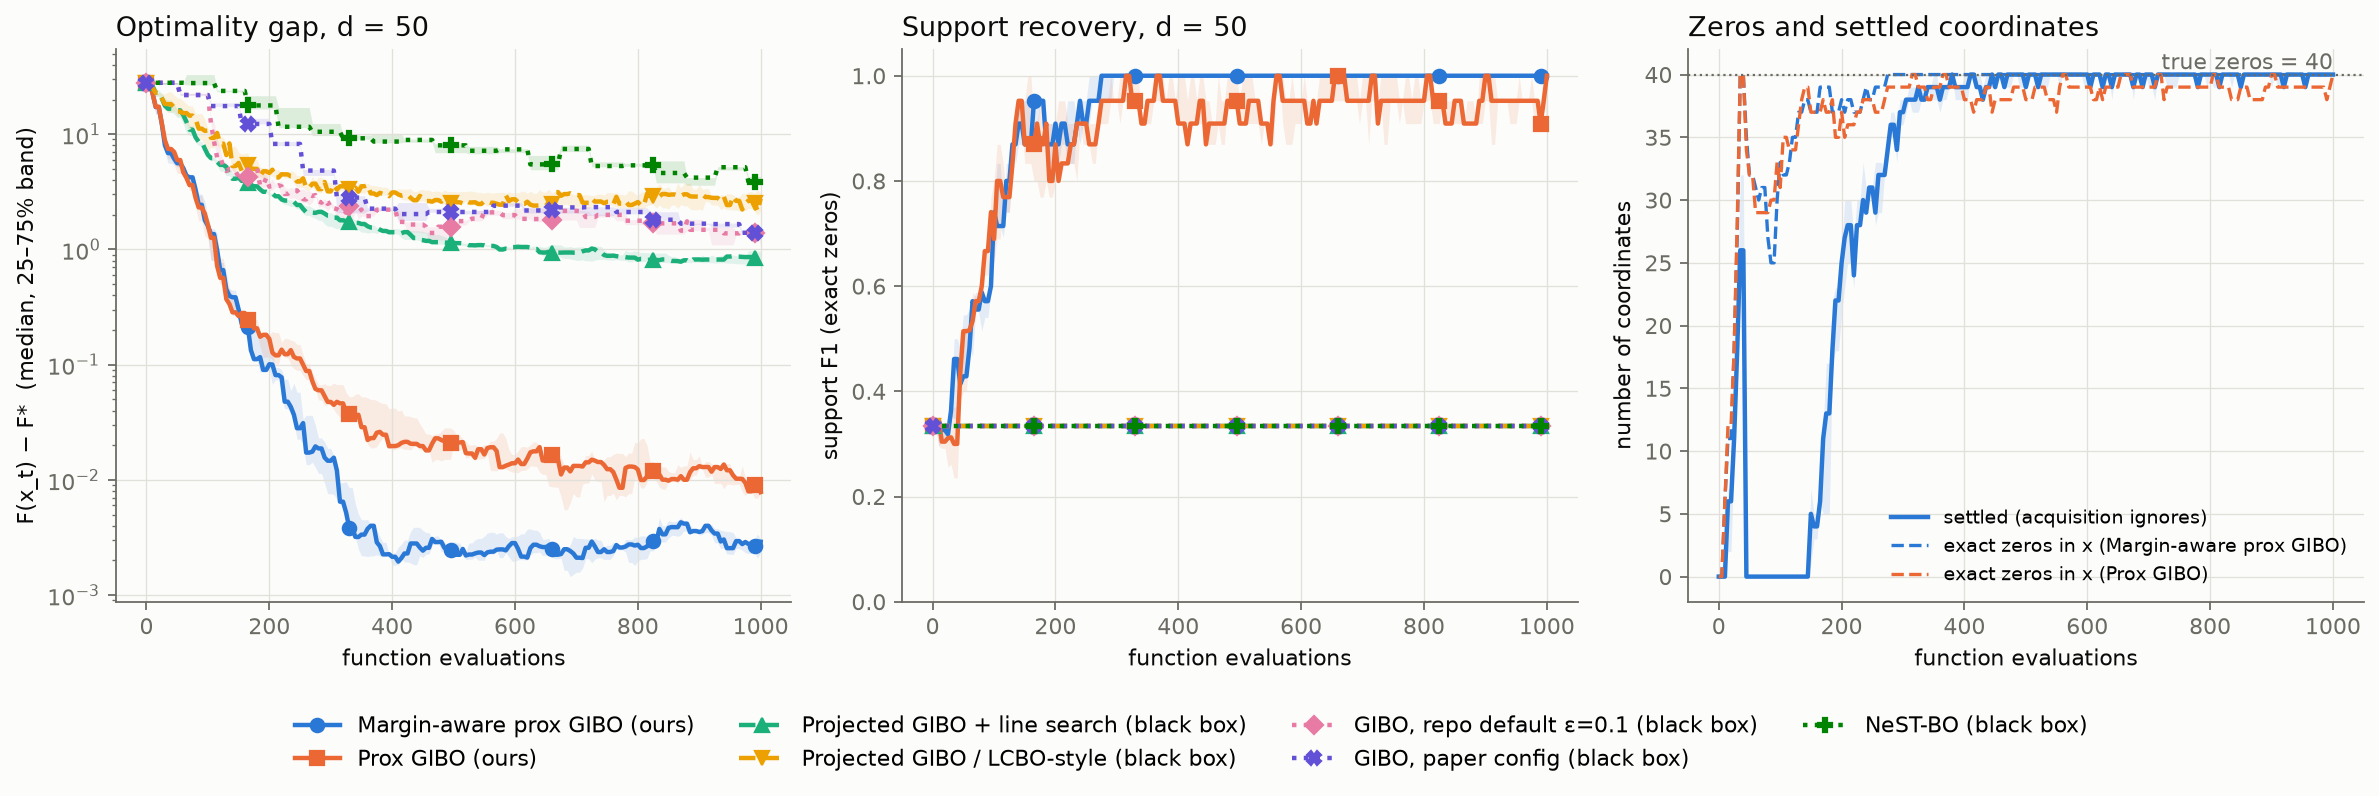
\includegraphics[width=\textwidth]{curves_d50.png}
\caption{$d=50$, median over 5 seeds with 25--75\% bands. Left: optimality gap. Middle: support F1. Right: exact zeros in $x_t$ (dashed) and
coordinates settled by the margin test (solid).}\label{fig:d50}
\end{figure}

Using $h$ explicitly gives final gaps two to three orders of magnitude smaller than every black-box method, together with exact support recovery.
The black-box methods never produce exact zeros. NeST-BO at $d=100$ was stopped after 10 hours at about 350 evaluations (gap 30--53, from 43--55).

\subsection{Scaling with $d$}\label{sec:exp-scaling}
\begin{figure}[h]
\centering
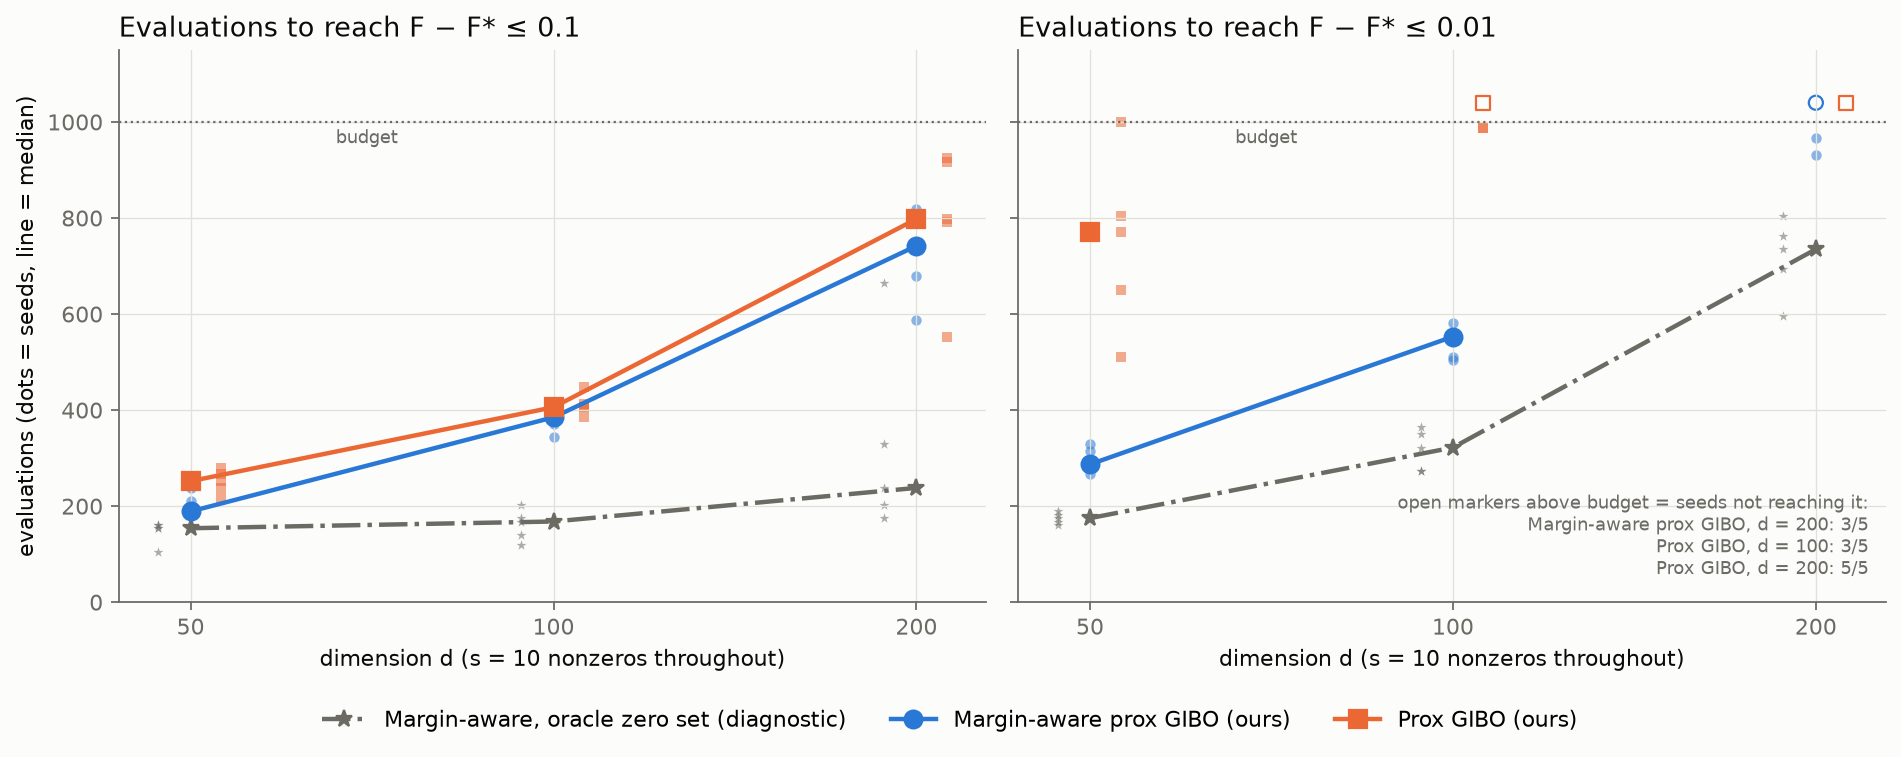
\includegraphics[width=0.92\textwidth]{scaling_prox_variants.png}
\caption{Evaluations to reach a gap of 0.1 (left) and 0.01 (right) as $d$ grows with $s=10$. Grey: diagnostic that is told the true zero set
(not a usable method).}\label{fig:scaling}
\end{figure}
With the real test, margin-aware needs $189\to385\to742$ evaluations to reach 0.1 for $d=50\to100\to200$, which is linear in $d$. The test fires late:
at $d=200$ the prox step produces the zeros within about 100 evaluations, but they are settled only after about 450. With the true zero set (grey)
the cost is $154\to168\to238$, nearly flat in $d$, so the weighting idea works and the bottleneck is the certificate. To reach 0.01 even the
diagnostic grows roughly linearly ($175\to322\to735$), which points to a second bottleneck in the final phase.

\subsection{Further checks}\label{sec:exp-other}
\begin{itemize}
\item \textbf{Noise-free evaluations}: margin-aware reaches a gap of $10^{-3}$ in all runs (308 evaluations at $d=50$, 525 at $d=100$).
\item \textbf{Condition number 100}, $d=50$: final gap 0.0030 (margin-aware) vs.\ 0.016 (prox-GIBO); everything is about $3\times$ slower.
\item \textbf{Proximal Newton} \citep{lee2014proxnewton}: we replaced the proximal-gradient step with a proximal-Newton step using the GP-mean Hessian,
with the subproblem solved by FISTA. It is worse everywhere (final gap 0.0049 vs.\ 0.0029 at condition number 10, 0.085 vs.\ 0.0030 at
condition number 100), because the GP Hessian has about 100\% relative error. With the \emph{true} Hessian, Newton gains nothing at condition
number 10 and about 30\% fewer evaluations at condition number 100.
\end{itemize}

\subsection{Benchmark from the GIBO and NeST-BO papers: Swimmer}\label{sec:exp-swimmer}
Swimmer is a MuJoCo \citep{todorov2012mujoco} locomotion task, used through Gymnasium \citep{towers2024gymnasium}, with a linear policy:
action $=Ws$, $W\in\R^{2\times8}$, so $d=16$. Linear policies are known to be competitive on such tasks \citep{mania2018ars}. Both GIBO and NeST-BO
report results on this benchmark \citep{muller2021gibo,tang2026nestbo}. We follow the NeST-BO setting: Swimmer-v5, box $[-10,10]^{16}$ (from the
NeST-BO code), start at the centre $x_0=0$, 10 initial Sobol points and batches of $M=d$ points for NeST-BO, a fixed environment seed, and
10 replicates. Here $f(x)=-(\text{episode return})$ and the budget is 300 episodes. We compare the original benchmark ($\lambda=0$) with a
sparse-controller version, $F=f+2\|x\|_1$. Our methods use step rule (ii), so they differ from GIBO only in how $h$ is handled.

\paragraph{Two metrics.}
\begin{itemize}
\item \emph{Best found}: the lowest $F$ among all evaluated points. This is the metric of the NeST-BO paper (``final best-found objective'',
median and IQR over 10 replicates).
\item \emph{Final iterate}: the point the method currently proposes. This is the relevant output for the sparse controller, because only
proximal iterates are exactly sparse; acquisition points are not.
\end{itemize}
NeST-BO's iterates oscillate much more than the others, so the two metrics differ most for NeST-BO.

\begin{table}[h]
\centering\small\setlength{\tabcolsep}{3.5pt}
\begin{tabular}{@{}clcccccc@{}}
\toprule
& & \multicolumn{2}{c}{Best found} & \multicolumn{4}{c}{Final iterate}\\\cmidrule(lr){3-4}\cmidrule(l){5-8}
$\lambda$ & Method & $F$ median (IQR) & Reward & $F$ median (IQR) & Reward & Nonzero gains & Stuck\\\midrule
0 & Prox-GIBO (ours) & $-337.0$ (98.6) & 337.0 & $-321.5$ (118.5) & 321.5 & 16 & 0/10\\
0 & Margin-aware prox-GIBO (ours) & $-334.4$ (52.1) & 334.4 & $-326.2$ (103.0) & 326.2 & 16 & 0/10\\
0 & GIBO & $-336.8$ (67.4) & 336.8 & $-328.8$ (203.0) & 328.8 & 16 & 1/10\\
0 & NeST-BO & $-279.2$ (44.8) & 279.2 & $-118.0$ (115.0) & 118.0 & 16 & 4/10\\
0 & LCBO-style & $-237.4$ (134.2) & 237.4 & $-118.7$ (146.2) & 118.7 & 16 & 4/10\\\midrule
2 & \textbf{Prox-GIBO (ours)} & $\mathbf{-318.1}$ (35.8) & 350.1 & $\mathbf{-308.7}$ (134.8) & 330.1 & \textbf{12} & 2/10\\
2 & \textbf{Margin-aware prox-GIBO (ours)} & $-316.7$ (95.0) & 350.7 & $-268.9$ (118.5) & 316.5 & \textbf{11} & 1/10\\
2 & GIBO & $-271.3$ (67.7) & 333.8 & $-238.1$ (77.3) & 303.8 & 16 & 0/10\\
2 & NeST-BO & $-242.7$ (53.1) & 306.2 & $-124.2$ (190.4) & 207.0 & 16 & 3/10\\
2 & LCBO-style & $-111.9$ (135.9) & 164.7 & $+21.7$ (158.4) & 33.2 & 16 & 8/10\\
\bottomrule
\end{tabular}
\caption{Swimmer, 10 replicates, 300 episodes. ``Reward'' is the episode return at the respective point (for $\lambda=0$, reward $=-F$).
``Stuck'' means a final-iterate reward below 100, the known poor local optimum. Nonzero gains are medians out of 16.}\label{tab:swimmer}
\end{table}

\begin{figure}[h]
\centering
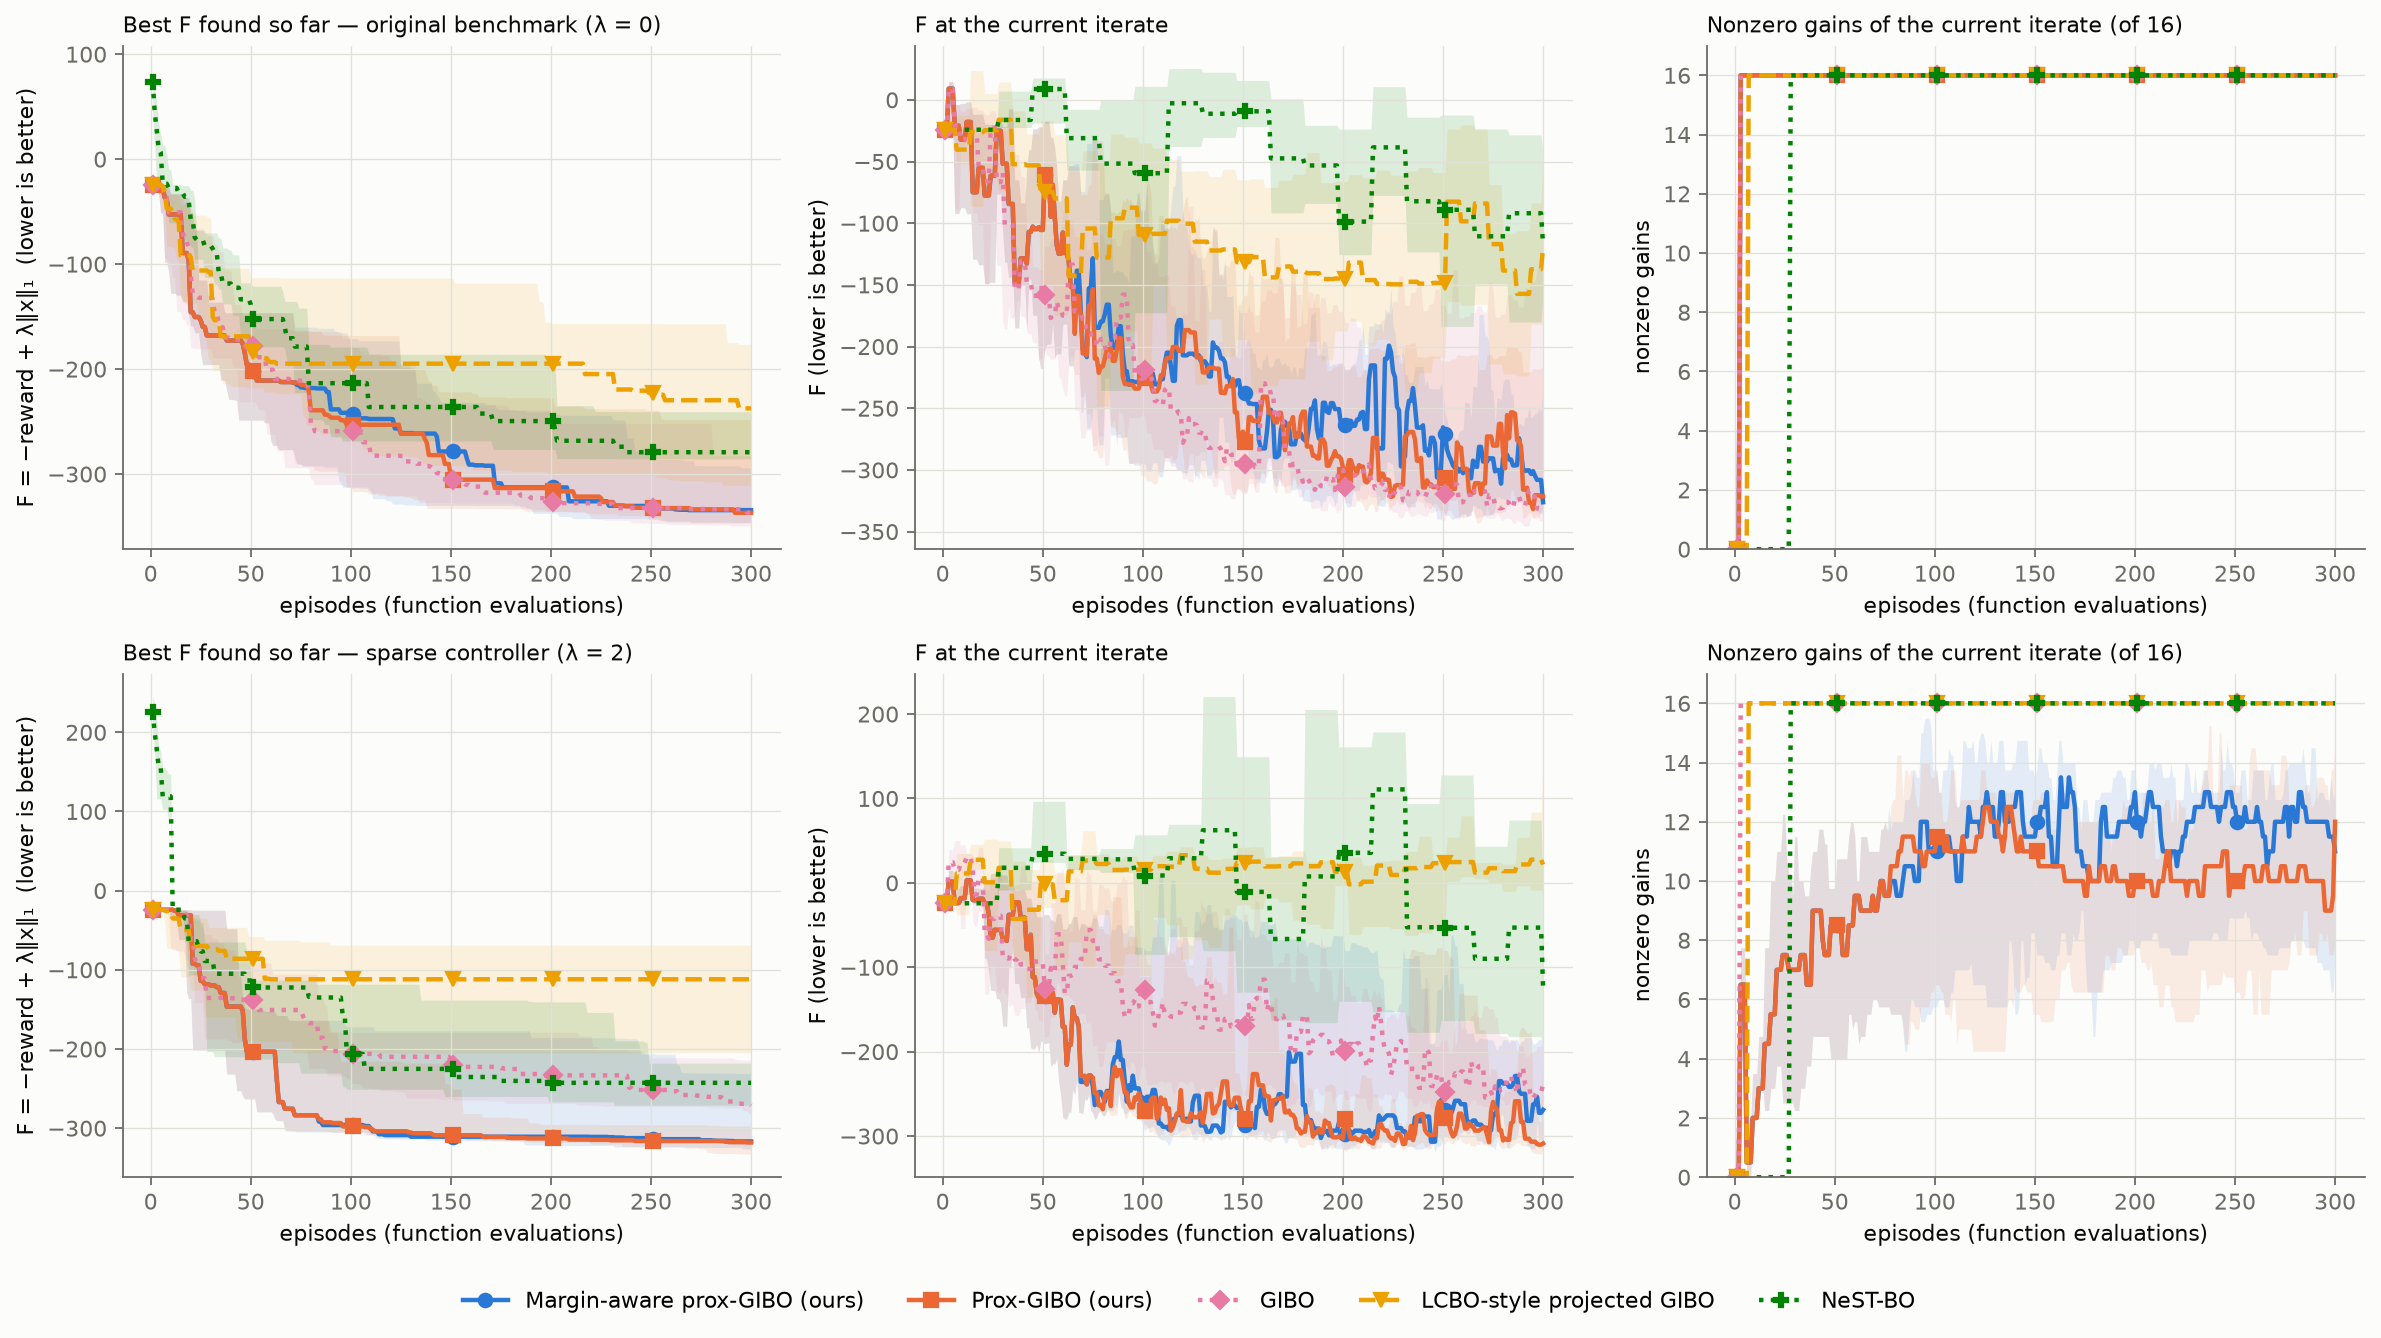
\includegraphics[width=\textwidth]{swimmer.png}
\caption{Swimmer, median over 10 replicates with 25--75\% bands. Top: $\lambda=0$. Bottom: $\lambda=2$. Left: best $F$ found so far.
Middle: $F$ at the current iterate. Right: nonzero gains of the current iterate.}\label{fig:swimmer}
\end{figure}

\paragraph{What the Swimmer study shows.}
\begin{itemize}
\item \textbf{Original benchmark ($\lambda=0$).} With $h=0$, prox-GIBO and margin-aware prox-GIBO are the same algorithm as GIBO. The small
differences between them come from floating-point non-determinism in a chaotic simulator. All three reach a best-found reward of about 335--337.
\item \textbf{Sparse controller ($\lambda=2$).} The proximal methods reach the best objective under both metrics: best-found $F$ of $-318$ and
$-317$, against $-271$ for GIBO and $-243$ for NeST-BO. Their final iterates use a median of 11--12 of the 16 gains, at a reward of 317--330,
while all black-box methods keep all 16 gains.
\item \textbf{Margin-aware} sampling brings no clear advantage over plain prox-GIBO at $d=16$, as expected.
\item \textbf{Comparison with the NeST-BO paper.} The paper reports a best-found objective of $-339.6$ (IQR 16.5) for NeST-BO on Swimmer
\citep{tang2026nestbo}; our runs give $-279.2$ (IQR 44.8). The difference is most likely due to the budget, which the paper does not state for
Swimmer and which we set to 300 episodes, and to settings our adapter may not reproduce exactly. Conversely, our GIBO ($-336.8$) does much better
than the GIBO numbers in that paper ($-183.9$), so the two GIBO implementations and settings also differ. These comparisons should be read
with this in mind. We have not tuned NeST-BO.
\item \textbf{Runtime.} With 11 runs sharing 12 CPU cores, one run took about 1--2 minutes for the GIBO-type methods and about 35--42 minutes
for NeST-BO, whose acquisition also targets Hessian information.
\end{itemize}

\section{Assessment and research plan}\label{sec:plan}

\begin{center}\small
\begin{tabular}{@{}L{0.33\linewidth}L{0.1\linewidth}L{0.5\linewidth}@{}}
\toprule
Hypothesis & Outcome & Evidence\\\midrule
(a) the support is identified and stable & yes & F1 $=1.00$ at all $d$ for margin-aware\\
(b) margin-aware beats plain prox by $\approx2\times$ & partly & 2.7--7$\times$ lower final gap; at $d=200$ the budget is too small for the 0.01 comparison\\
(c) cost grows with $s$, not $d$ & not yet & the certificate fires late; with the true zero set the cost is nearly flat in $d$\\
\bottomrule
\end{tabular}
\end{center}

\paragraph{Known issues.} The GP gradient's error bars are 2--4$\times$ too optimistic near $x^\star$. 3 of 140 runs show a jump on the very last
iteration. ARD length scales of coordinates that are no longer sampled drift upward, which required a trust region.

\paragraph{Theory.}
\begin{enumerate}[label=(T\arabic*)]
\item Convergence of prox-GIBO as an inexact proximal-gradient method (\cref{sec:inexact}), with the error $e_k$ bounded with high probability by
GP confidence bounds under an RKHS assumption on $f$ \citep{srinivas2010ucb}.
\item High-probability support identification via \cref{prop:ident}, and the sample complexity it implies.
\item A query complexity for margin-aware acquisition that depends on $s$ and the margin $\min_i\delta_i$ rather than $d$. This needs a
certificate that fires early enough.
\end{enumerate}

\paragraph{Method and experiments.}
\begin{enumerate}[label=(M\arabic*)]
\item A better settling certificate: pool evidence across iterations, or use a sequential test, or calibrate $\kappa$.
\item An adaptive batch size driven by the weighted gain, so that fewer active coordinates also means fewer evaluations per iteration.
\item Freeze settled coordinates in the step, and add a step safeguard.
\item Extensions: group lasso (case A, already implemented), a total-variation problem with a primal--dual step (case C), and a non-quadratic
synthetic problem.
\item Baselines: SEBO \citep{liu2023sebo}; more seeds and larger $d$ on the cluster.
\end{enumerate}

\paragraph{Reproducibility.} Code in \texttt{prox\_bo/} and \texttt{experiments/}. All seeds are fixed, and raw results (NPZ/JSON) are in \texttt{results/}.

\bibliographystyle{plainnat}
\bibliography{refs_opt,refs_bo}

\end{document}
